\documentclass[color=usenames,dvipsnames]{beamer}\usepackage[]{graphicx}\usepackage[]{color}
% maxwidth is the original width if it is less than linewidth
% otherwise use linewidth (to make sure the graphics do not exceed the margin)
\makeatletter
\def\maxwidth{ %
  \ifdim\Gin@nat@width>\linewidth
    \linewidth
  \else
    \Gin@nat@width
  \fi
}
\makeatother

\definecolor{fgcolor}{rgb}{0.345, 0.345, 0.345}
\newcommand{\hlnum}[1]{\textcolor[rgb]{0.686,0.059,0.569}{#1}}%
\newcommand{\hlstr}[1]{\textcolor[rgb]{0.192,0.494,0.8}{#1}}%
\newcommand{\hlcom}[1]{\textcolor[rgb]{0.678,0.584,0.686}{\textit{#1}}}%
\newcommand{\hlopt}[1]{\textcolor[rgb]{0,0,0}{#1}}%
\newcommand{\hlstd}[1]{\textcolor[rgb]{0.345,0.345,0.345}{#1}}%
\newcommand{\hlkwa}[1]{\textcolor[rgb]{0.161,0.373,0.58}{\textbf{#1}}}%
\newcommand{\hlkwb}[1]{\textcolor[rgb]{0.69,0.353,0.396}{#1}}%
\newcommand{\hlkwc}[1]{\textcolor[rgb]{0.333,0.667,0.333}{#1}}%
\newcommand{\hlkwd}[1]{\textcolor[rgb]{0.737,0.353,0.396}{\textbf{#1}}}%
\let\hlipl\hlkwb

\usepackage{framed}
\makeatletter
\newenvironment{kframe}{%
 \def\at@end@of@kframe{}%
 \ifinner\ifhmode%
  \def\at@end@of@kframe{\end{minipage}}%
  \begin{minipage}{\columnwidth}%
 \fi\fi%
 \def\FrameCommand##1{\hskip\@totalleftmargin \hskip-\fboxsep
 \colorbox{shadecolor}{##1}\hskip-\fboxsep
     % There is no \\@totalrightmargin, so:
     \hskip-\linewidth \hskip-\@totalleftmargin \hskip\columnwidth}%
 \MakeFramed {\advance\hsize-\width
   \@totalleftmargin\z@ \linewidth\hsize
   \@setminipage}}%
 {\par\unskip\endMakeFramed%
 \at@end@of@kframe}
\makeatother

\definecolor{shadecolor}{rgb}{.97, .97, .97}
\definecolor{messagecolor}{rgb}{0, 0, 0}
\definecolor{warningcolor}{rgb}{1, 0, 1}
\definecolor{errorcolor}{rgb}{1, 0, 0}
\newenvironment{knitrout}{}{} % an empty environment to be redefined in TeX

\usepackage{alltt}
%\documentclass[color=usenames,dvipsnames,handout]{beamer}

%\usepackage[roman]{../pres1}
\usepackage[sans]{../pres1}




\IfFileExists{upquote.sty}{\usepackage{upquote}}{}
\begin{document}



\begin{frame}[plain]
  \begin{center}
    {\huge \bf Sampling and Estimation \par}
    \vspace{0.5cm}
    \vfill
      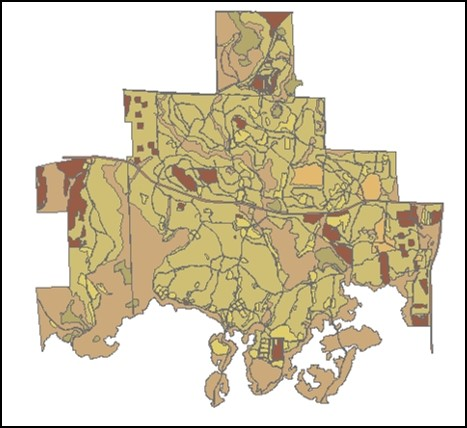
\includegraphics[height=4.2cm,keepaspectratio]{figs/map} \hfill %\hspace{0.5cm}
      \fbox{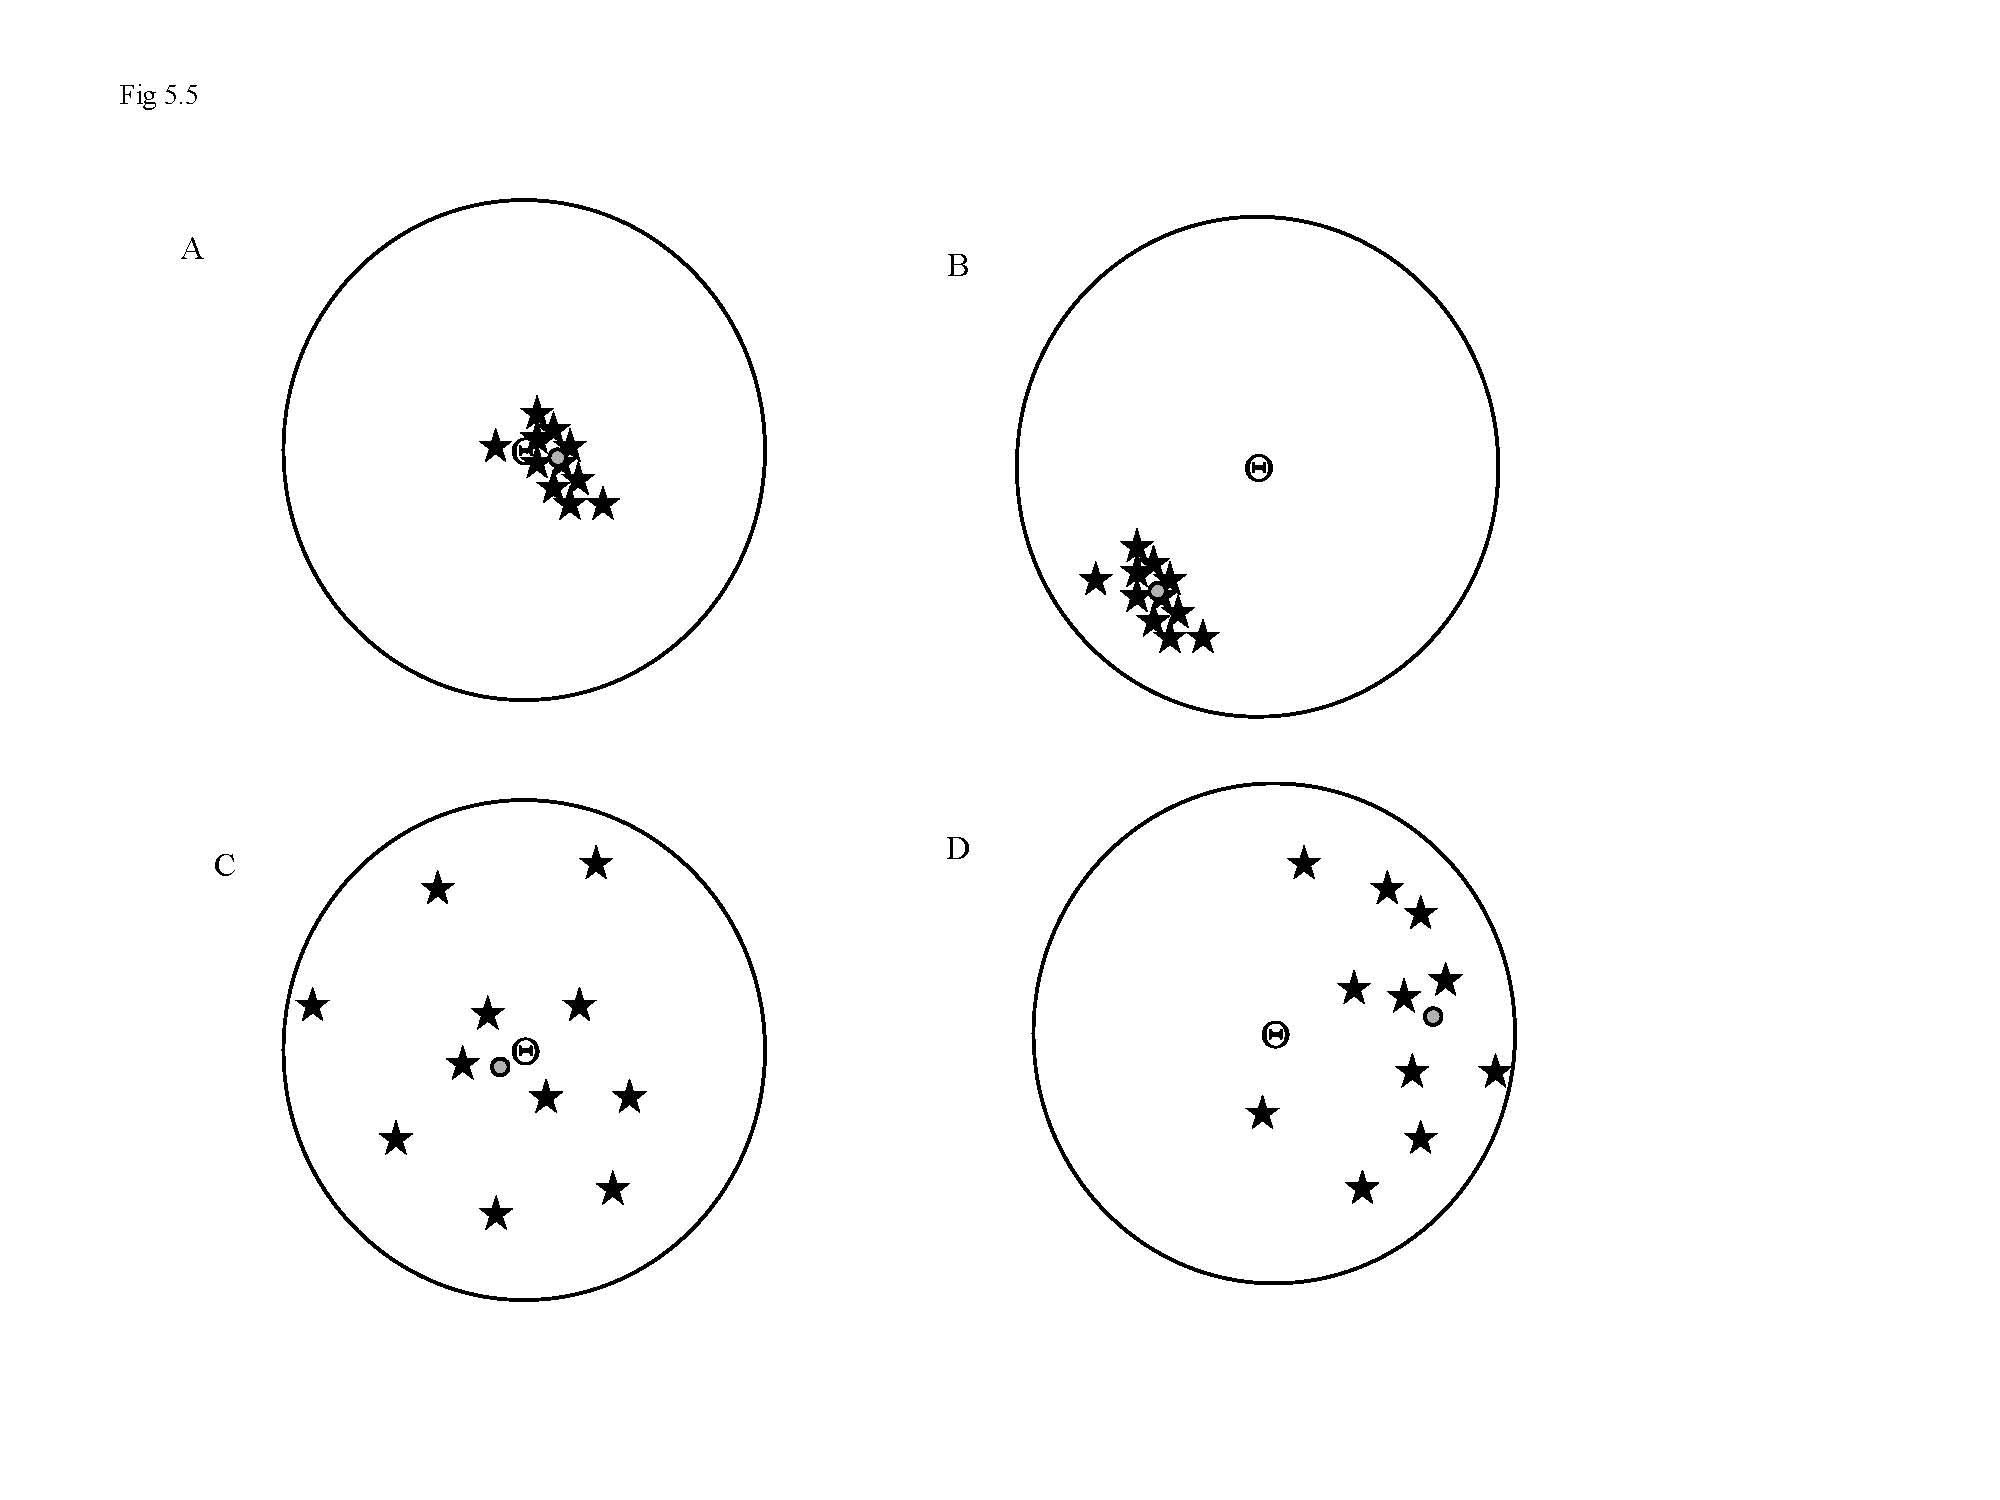
\includegraphics[height=4.2cm,keepaspectratio,trim = 0mm
        0mm 0mm 0mm, clip]{figs/bulls-eye.jpg}}
  \end{center}
\end{frame}




\section{Introduction}



\begin{frame}
  \frametitle{Model parameters}
  \large
  {\bf Key concepts}
  \begin{itemize}%[<+->]
    \item<1-> All models include parameters (e.g., $N$, $r$, $K$, etc\dots)
    \item<2-> Parameters are almost never known. Why?
      \begin{itemize}
        \large
        \item<3-> We usually have to sample
        \item<3-> Animals are hard to detect
      \end{itemize}
    \item<4-> Good sampling designs yield accurate %reliable
      estimates of unknown parameters
  \end{itemize}
\end{frame}




\begin{frame}
  \frametitle{Parameters, estimates, and statistics}
  \large
  {\bf Parameter}                                                       \\
  A characteristic of a population \par
  \vspace{0.7cm}
  \uncover<2->{
  {\bf Statistic}                                                       \\
  A characteristic of a dataset (often used to estimate a parameter) \par
  }
  \vfill %\vspace{0.7cm}
  \uncover<3->{
  \begin{center}
    \large
  %   \begin{tabular}{lm{2cm}m{2cm}}
  \begin{tabular}{lcc}
    \hline
    %                         & Sample statistic & Population parameter \\
                              & Population       & Parameter           \\
                              & parameter        & estimate            \\
    \hline
    Population size           & $N_t$      & $\hat{N}_t$                  \\
    Growth rate               & $r$        & $\hat{r}$                  \\
    Occurrence probability    & $\psi$     & $\hat{\psi}$               \\
    \hline
  \end{tabular}
  \end{center}
  }
\end{frame}



\begin{frame}
  \frametitle{How do you get accurate estimates?}
  \large
%  {Reliable estimates are accurate repeatable and defensible \par}
%  \vspace{0.5cm}
%  \uncover<2->{{\bf Reliable estimates achievable with good sampling designs \par}}
%  \vspace{0.5cm}
  \uncover<1->{{\bf Properties of a good design:}}
  \begin{enumerate}[(1)]
    \item<2-> Clearly defined objective, in terms of:
      \begin{itemize}%[<3->]
        \large
        \item Parameter(s) that will be estimated
        \item Population of interest
        \item Criteria for reliability (e.g., precision)
        \item Practical constraints (e.g., costs)
      \end{itemize}
    \item<5-> Replication
%      \begin{itemize}
%        \item Sample size
%      \end{itemize}
    \item<6-> Randomization
    \item<7-> Controls (when conducting an experiment)
  \end{enumerate}
  \vfill
  \uncover<3->{{\bf Bad objective}: ``Quantify the abundance of tigers in India'' \\}
  \vfill
  \uncover<4->{{\bf Better objective}: ``Obtain an unbiased estimate of tiger density on the Corbett Tiger Reserve during July 2009, with a coefficient of variation $<$25\% for under \$5,000.''}
\end{frame}




\begin{frame}
  \frametitle{Defining the population}
  \large
  {\bf Target population} \\
  The population of interest. Should be defined in terms of time and
  space. \par
  \pause
  \vspace{1cm}
  {\bf Sampled population} \\
  The sampled portion of the population of interest, usually defined
  in terms of the sample units (such as plots, quadrats, etc.).
\end{frame}





\begin{frame}
  \frametitle{Accuracy}
%  \large
  {\bf \large Accuracy has two components: \par}
  \begin{enumerate}[\bf (1)]
    \normalsize
    \item {\bf Bias}: The difference between the average estimate and
      the true parameter \par
    \item {\bf Variance}: The variability of the estimates.
  \end{enumerate}
  \pause
  \centering
  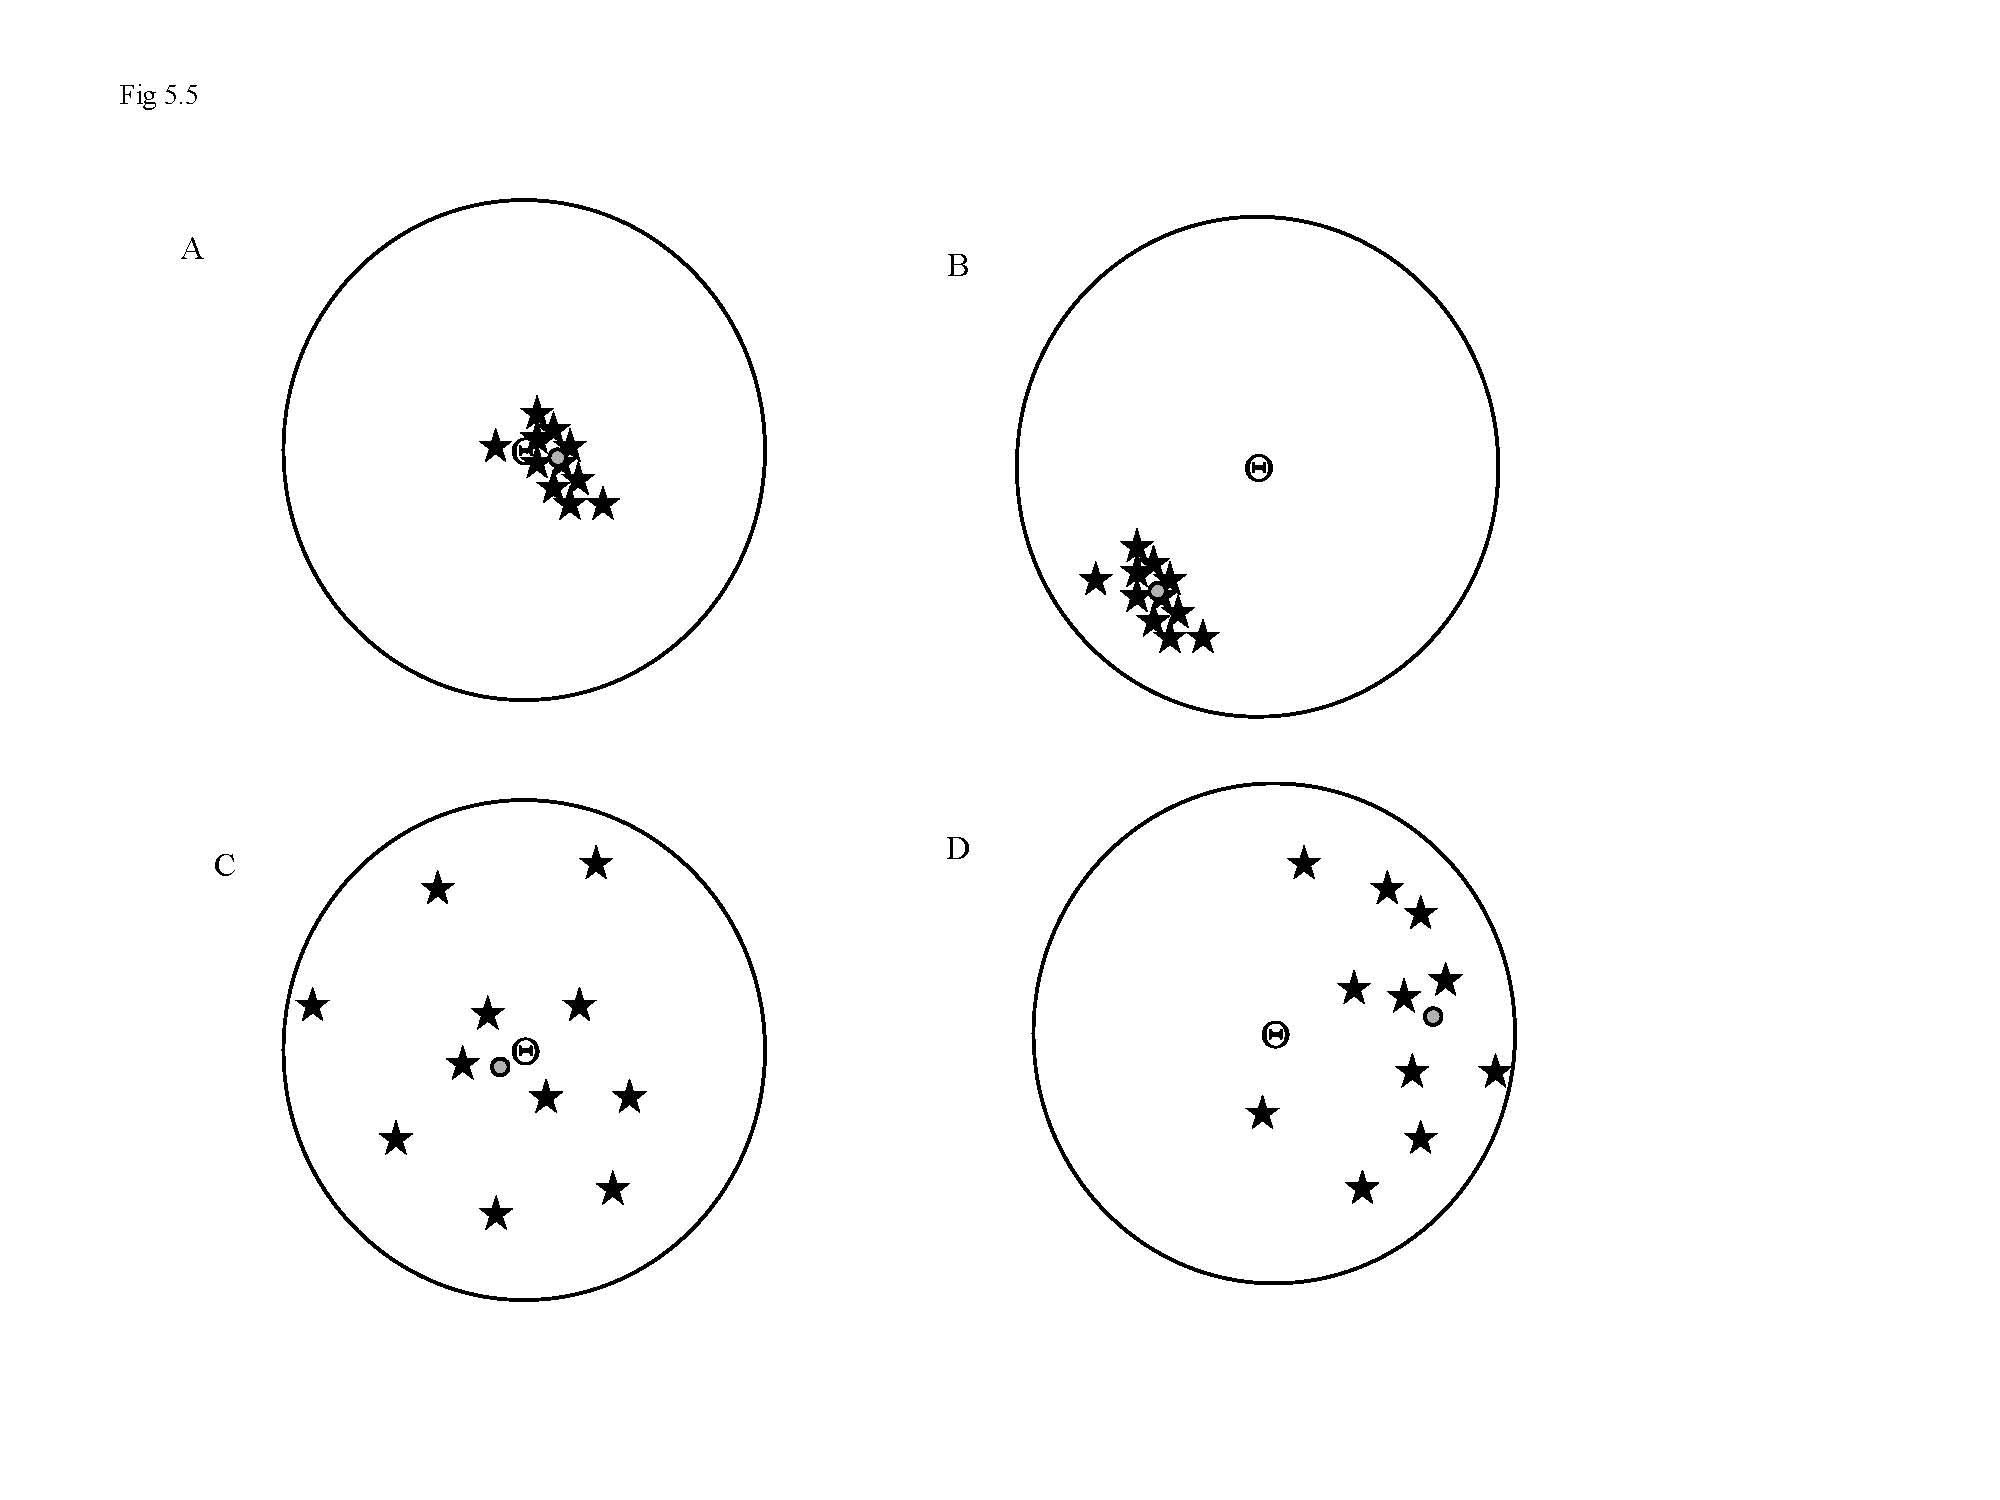
\includegraphics[width=0.65\textwidth]{figs/bulls-eye.jpg} \\
\end{frame}






\section{Sampling}



\begin{frame}
  \frametitle{How do we reduce variance?}
  \pause
  \begin{center}
    \Huge Huge sample size
  \end{center}
\end{frame}





\begin{frame}[fragile]
  \frametitle{Effect of sample size}
%  \bf
  Suppose we want to estimate the height of students on campus, and we
  have enough resources to repeat a survey many times. \\
  \centering
  Each point below is an estimate. \\
  \vfill



%\vspace{-0.8cm}
\begin{center}
  \includegraphics<1 | handout:0>[width=\textwidth]{figs/sample-size/f1}
  \includegraphics<2 | handout:0>[width=\textwidth]{figs/sample-size/f2}
  \includegraphics<3 | handout:0>[width=\textwidth]{figs/sample-size/f3}
  \includegraphics<4 | handout:0>[width=\textwidth]{figs/sample-size/f4}
  \includegraphics<5 | handout:0>[width=\textwidth]{figs/sample-size/f5}
  \includegraphics<6 | handout:0>[width=\textwidth]{figs/sample-size/f6}
  \includegraphics<7 | handout:0>[width=\textwidth]{figs/sample-size/f7}
  \includegraphics<8 | handout:0>[width=\textwidth]{figs/sample-size/f8}
  \includegraphics<9 | handout:0>[width=\textwidth]{figs/sample-size/f9}
  \includegraphics<10->[width=\textwidth]{figs/sample-size/f100} \par
%  \vspace{0.4cm}
  \vfill
 % \large
  \uncover<11>{The standard deviation of the sampling distribution is
    called the standard error (SE)}
\end{center}
\end{frame}






\begin{frame}
  \frametitle{How do we reduce bias?}
  \pause
  \begin{center}
    \Huge Randomization
  \end{center}
\end{frame}










% \begin{frame}
%   \frametitle{How do we get an unbiased estimator?}
%   \begin{enumerate}[(1)]
%     \item Design-based approaches
%       \begin{itemize}
%         \item Random sampling
%         \item Stratified random sampling
%         \item Cluster sampling
%         \item etc\dots
%       \end{itemize}
%     \item Model-based approaches
%   \end{enumerate}
% \end{frame}





%% \begin{frame}
%%   \frametitle{Standard sampling designs}
%% %  \Large
%% %  \begin{itemize}[<+->]
%% %    \item<1-> Simple random sampling
%%   \large
%%   {\bf Simple random sampling}
%%   \begin{itemize}
%%     \item All sample units have the same inclusion probability
%%     \item Easiest and most reliable method
%%     \item But not always cost effective
%%   \end{itemize}
%% %    \item<2-> Stratified random sampling
%%   \pause
%%   {\bf Stratified random sampling}
%%   \begin{itemize}
%%     \item Useful when the study area is characterized by several
%%       homogeneous regions
%%     \item Regions with higher variability should be sampled more
%%         intensively than regions with low variability
%%     \item Often more cost effective than simple random sampling
%%   \end{itemize}
%% %    \item<3-> Systematic sampling
%%     \pause
%%   {\bf Systematic sampling}
%%   \begin{itemize}
%%     \item Could involve sampling on a regular grid
%%     \item Dangerous if grid corresponds to environmental patterns
%%   \end{itemize}
%% \end{frame}




\begin{frame}
  \frametitle{Standard sampling designs}
  \large
  {\centering \bf \Large \color{RoyalBlue}{Simple random sampling} \par}
  \vfill
  \begin{columns}
    \large
    \begin{column}{0.6\textwidth}
      \begin{itemize}[<+->]
        \item All sample units have the same inclusion probability
        \item Easiest and most reliable method
        \item But not always cost effective
      \end{itemize}
    \end{column}
    \begin{column}{0.4\textwidth}
      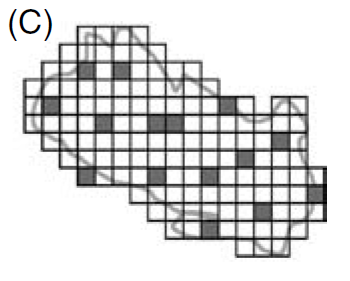
\includegraphics[width=\textwidth]{figs/designC}
    \end{column}
  \end{columns}
\end{frame}


%% \begin{frame}
%%   \frametitle{Standard sampling designs}
%%   \large
%%   {\bf Stratified random sampling}
%%   \begin{itemize}
%%     \item Useful when the study area is characterized by several
%%       homegeneous regions
%%     \item Regions with higher variability should be sampled more
%%       intensively than regions with low variability
%%     \item Often more cost effective than simple random sampling
%%    \end{itemize}
%% \end{frame}


\begin{frame}
  \frametitle{Standard sampling designs}
  \large
  {\centering \bf \Large \color{RoyalBlue}{Stratified random sampling} \par}
  \vfill
  \begin{columns}
    \large
    \begin{column}{0.6\textwidth}
      \begin{itemize}[<+->]
        \item Useful when study area is characterized by several
          homogeneous regions
        \item Regions with higher variability should be sampled more
          intensively than regions with low variability
        \item Often more cost effective than simple random sampling
      \end{itemize}
    \end{column}
    \begin{column}{0.4\textwidth}
      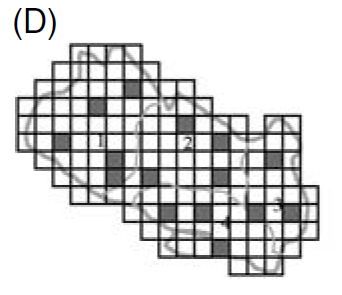
\includegraphics[width=\textwidth]{figs/designD}
    \end{column}
  \end{columns}
\end{frame}



%% \begin{frame}
%%   \frametitle{Standard sampling designs}
%%   \large
%%   {\bf Systematic sampling}
%%   \begin{itemize}
%%     \item Could involve sampling on a regular grid
%%     \item Dangerous if grid corresponds to environmental patterns
%%   \end{itemize}
%% \end{frame}



\begin{frame}
  \frametitle{Standard sampling designs}
  \large
  {\centering \bf \Large \color{RoyalBlue}{Systematic sampling} \par}
  \vfill
  \begin{columns}
    \large
    \begin{column}{0.6\textwidth}
      \begin{itemize}[<+->]
        \item Sample units are selected according to a regular,
          ordered scheme with the first unit being sampled randomly.
        \item Easy to implement in the field
        \item Potentially dangerous because sample unit spacing could
          coincide with natural spacing of environmental features
      \end{itemize}
    \end{column}
    \begin{column}{0.4\textwidth}
      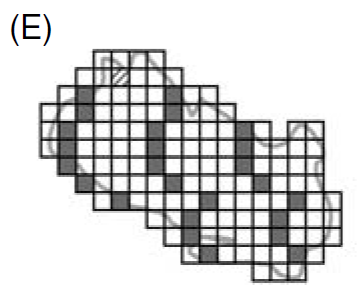
\includegraphics[width=\textwidth]{figs/designE}
    \end{column}
  \end{columns}
\end{frame}






%% \begin{frame}
%%    \frametitle{Yellow-rumped Warblers at Whitehall}
%%    \begin{center}
%%      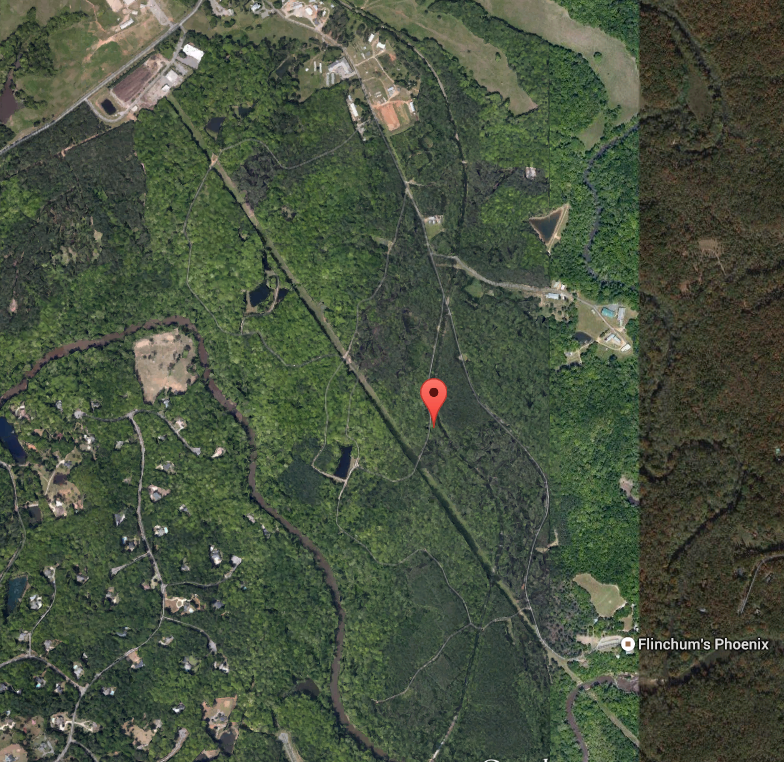
\includegraphics[width=0.7\textwidth]{figs/Whitehall}
%%    \end{center}
%% \end{frame}


% \begin{frame}
%   \frametitle{White-tailed deer in South Florida}
%   {\bf Objective:} Determine the impacts of hydrology, hunting, and
%   predation on white-tailed deer abundance and trends. \par
%   \begin{itemize}
%     \item The study area is the red rectangle
%     \item Water depth increases from west to east
%     \item No hunting allowed in FPNWR
%     \item Panthers potentially everywhere
%     \item You have a \$500,000 budget
%   \end{itemize}
%   \vfill
%   {\bf Question:} How would you design this study?
% %  \vfill
%    \begin{center}
%      \fbox{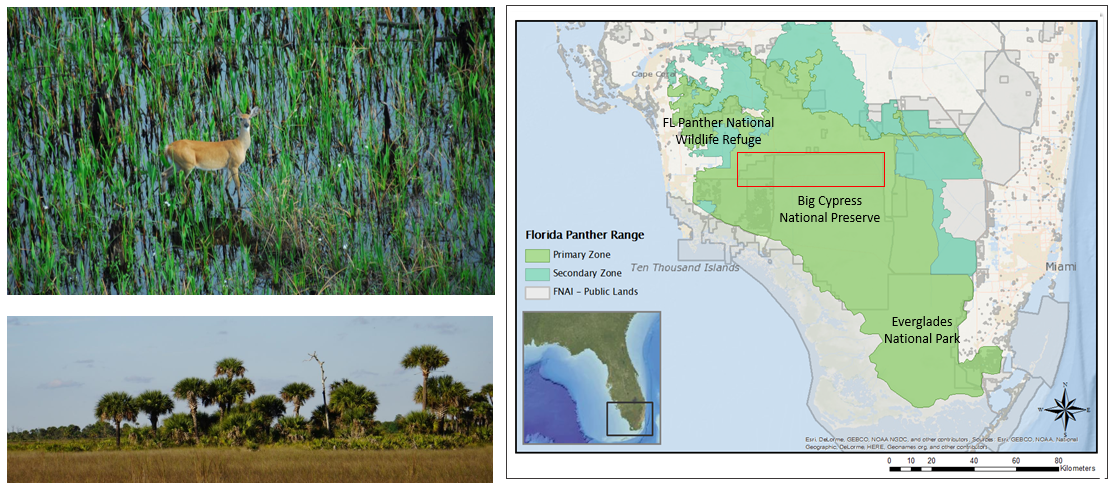
\includegraphics[width=0.7\textwidth]{figs/FL-deer-study}}
%    \end{center}
% \end{frame}



\begin{frame}
  \frametitle{Summary}
  \Large
  {\bf Main points}
  \begin{itemize}
    \item We have to estimate model parameters
    \item Reliable estimates require good sampling design
    \item Replication reduces variance
    \item Randomization reduces bias
  \end{itemize}
\end{frame}






%\begin{frame}
%  \frametitle{Golden-winged warblers in Costa Rica}
%  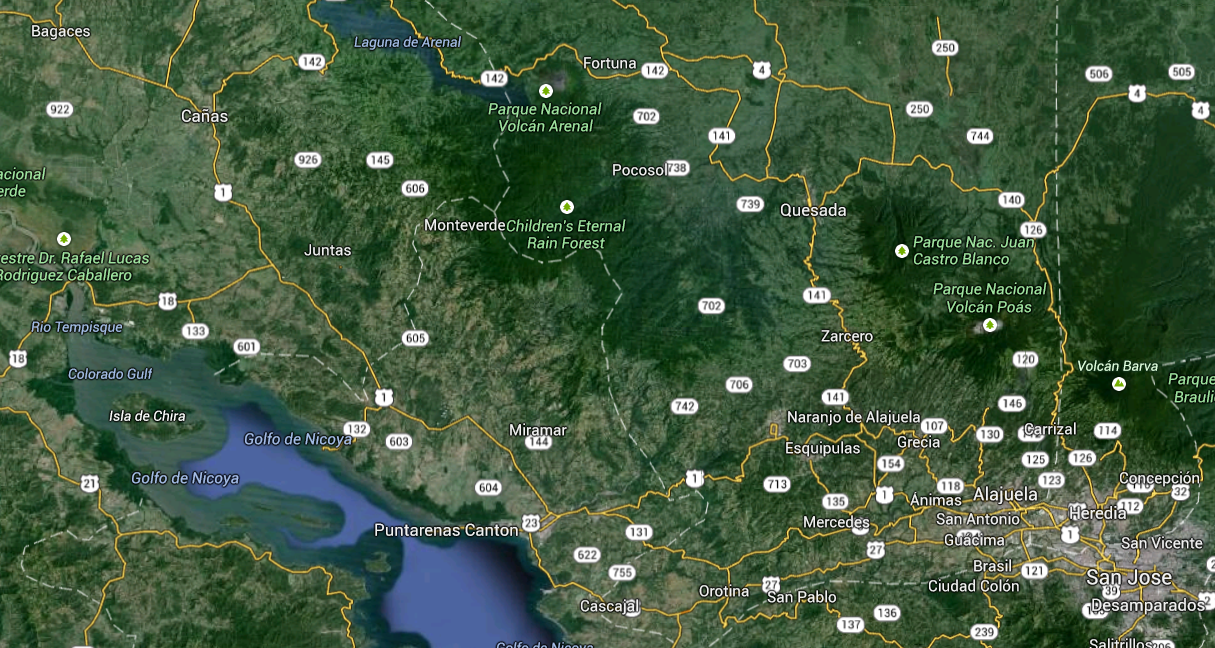
\includegraphics[width=\textwidth]{figs/Costa-Rica}
%\end{frame}










%\section{Detection probability}



%\begin{frame}
%  \frametitle{Detection probability}

%\end{frame}







\end{document}
